\documentclass[12pt]{article}

%packages
\usepackage{graphicx}
\usepackage{amsmath}
\usepackage{mathdots}
\usepackage{amsthm}
\usepackage{amssymb}
\usepackage[dvips]{color}
\usepackage{fancyhdr}
\usepackage{pstricks}
\usepackage{pst-node}
\pagenumbering{arabic}
\usepackage{hyperref}
\usepackage{lscape}
%Margins etc...
\setlength{\textheight}{240mm}
\setlength{\topmargin}{-17mm} \setlength{\oddsidemargin}{-4mm}
\setlength{\textwidth}{166mm} \setlength{\parindent}{0mm}
\setlength{\marginparsep}{9mm} \setlength{\parskip}{3mm}

\begin{document}
\begin{center}
\Huge{Queueing Theory Exercise Sheet Solutions}
\end{center}

\begin{enumerate}
\item Fill in the gaps in the following table:
\begin{center}
\begin{tabular}{c|c|c|c|c}
\hline
Statistic& Notation & $M/M/1$ & $M/M/2$ & $M/M/k$ \\\hline
Number of people in queue  & $L_q$ &   ${\rho^2\over 1-\rho}$       & ${2\rho^3\over 1-\rho^2}$  &  ${\left(\lambda\over \mu \right)^{k+1}\pi_0\over kk!\left(1-{\lambda\over k\mu} \right)^2}$    \\
Number of people in system & $L_c$ &   ${\rho\over 1-\rho}$       &   ${2\rho\over 1-\rho^2}$  &  ${\left(\lambda\over \mu \right)^{k+1}\pi_0\over kk!\left(1-{\lambda\over k\mu} \right)^2}+{\lambda\over \mu}$  \\
Average waiting time in queue & $W_q$ &    ${\rho\over \mu(1-\rho)}$    & ${\rho^2\over\mu( 1-\rho^2)}$ &  ${\left(\lambda\over \mu \right)^{k}\pi_0\over kk!\left(1-{\lambda\over k\mu} \right)^2\mu}$       \\
Average time in system & $W_c$ &   ${1\over \mu(1-\rho)}$       &${1\over\mu( 1-\rho^2)}$ &${\left(\lambda\over \mu \right)^{k}\pi_0\over kk!\left(1-{\lambda\over k\mu} \right)^2\mu}+{1\over \mu}$
\end{tabular}
\end{center}

\item
    \begin{itemize}
        \item FIFO:
        $$\begin{array}{@{}r@{\;}c@{\;}l@{}}
        \text{Total waiting time}&=&0+1+(1+2)+(1+2+3)+\dots+(1+2+3+\dots+(n-1))\\[2mm]
                                 &=&\sum_{k=1}^{n-1}\sum_{j=0}^kj=\sum_{k=1}^{n-1}{k(k+1)\over2}\\[2mm]
                                 &=&{1\over2}\left(\sum_{k=1}^{n-1}k^2+\sum_{k=1}^{n-1}k\right)\\[2mm]
                                 &=&{1\over2}\left({(n-1)n(2n-1)\over 6}+{n(n-1)\over2}\right)\\[2mm]
                                 &=&{1\over2}\left({(n-1)n(2n+2)\over 6}\right)={(n-1)n(n+1)\over 6}
        \end{array}$$
        However a total of $n$ customers are served thus:
        $$W_q={(n-1)(n+1)\over 6}={n-1^2\over 6}$$ as required.
        \item LIFO
         $$\begin{array}{@{}r@{\;}c@{\;}l@{}}
        \text{Total waiting time}&=&0+n+(n+(n-1))+\dots+(n+\dots+2)\\[2mm]
                                 &=&\sum_{k=0}^{n-2}\sum_{j=0}^k(n-j)=\sum_{k=0}^{n-2}\sum_{j=n-k}^nj=\sum_{k=0}^{n-2}\left(\sum_{j=0}^nj-\sum_{j=0}^{n-k-1}j\right)\\[2mm]
                                 &=&\sum_{k=0}^{n-2}\left({n(n+1)\over2}-{(k-n)(1+k-n)\over2}\right)=\sum_{k=0}^{n-2}{(k+1)(2n-k)\over2}\\[2mm]
                                 &=&{1\over2}\left(-\sum_{k=0}^{n-2}k^2+(2n-1)\sum_{k=0}^{n-2}k+\sum_{k=0}^{n-2}2n\right)\\[2mm]
                                 &=&{1\over2}\left(-{(n-2)(n-1)(2n-3)\over6}+{(n-2)(n-1)(2n-1)\over2}+2n(n-1)\right)={(n-1)n(n+1)\over 3}
        \end{array}$$
        However a total of $n$ customers are served thus:
        $$W_q={(n-1)(n+1)\over 3}={n-1^2\over 3}$$ as required.
    \end{itemize}


\item We have:
$$\begin{array}{@{}r@{\;}c@{\;}l@{}}
E(T)&=&\sum_{n=0}^\infty{n(\lambda t)^ne^{-\lambda t}\over n!}\\[2mm]
    &=&e^{-\lambda t}\sum_{n=0}^\infty{(\lambda t)^n\over (n-1)!}\\[2mm]
    &=&\lambda te^{-\lambda t}\sum_{n=0}^\infty{(\lambda t)^{n-1}\over (n-1)!}\\[2mm]
    &=&\lambda te^{-\lambda t}e^{\lambda t}\\[2mm]
\end{array}$$
  as required.\\

5 minutes $\Leftrightarrow$ ${1\over 12}$ hours. Thus, $\lambda t={24\over12}=2$.


$$\begin{array}{@{}r@{\;}c@{\;}l@{}}
P(X=0)&=&e^{-2}\approx .135335\\[2mm]
P(X=1)&=&{2e^{-2}\over1}\approx .270671\\[2mm]
P(X=2)&=&{2^2e^{-2}\over2}\approx .270671\\[2mm]
P(X=3)&=&{2^3e^{-2}\over6}\approx .180447\\[2mm]
\end{array}$$

We have: $$P(X\geq 4)=1-P(X\leq 3)=1-P(X=3)-P(X=2)-P(X=1)-P(X=0)\approx.142877$$

\item We have:
$$\begin{array}{@{}r@{\;}c@{\;}l@{}}
E(T)&=&\int_{0}^{\infty}\lambda te^{-\lambda t}dt\\[2mm]
    &=&\left.-{(\lambda t)e^{-\lambda t}\over \lambda}\right|_{0}^\infty+\int_{0}^{\infty}e^{-\lambda t}dt\\[2mm]
    &=&\left.-{e^{-\lambda t}\over \lambda}\right|_{0}^\infty={1\over \lambda}\\[2mm]
\end{array}$$
  as required.\\
  By definition: $F(x)=P(X\leq x)=\int_{0}^{\infty}\lambda e^{-\lambda t}dt=1-e^{-\lambda x}$. We have $\lambda=36$ which gives:

$$\begin{array}{@{}r@{\;}c@{\;}l@{}}
P(X\leq{1\over60})&=&1-e^{-36\over 60}\approx .451188\\[2mm]
P(X\leq{1\over30})&=&1-e^{-36\over 30}\approx .698806\\[2mm]
P(X\leq{1\over30})&=&1-P(X\leq{1\over30})=e^{-36\over 30}\approx .301194\\[2mm]
\end{array}$$

\item

The Markov chain is given:
\begin{center}
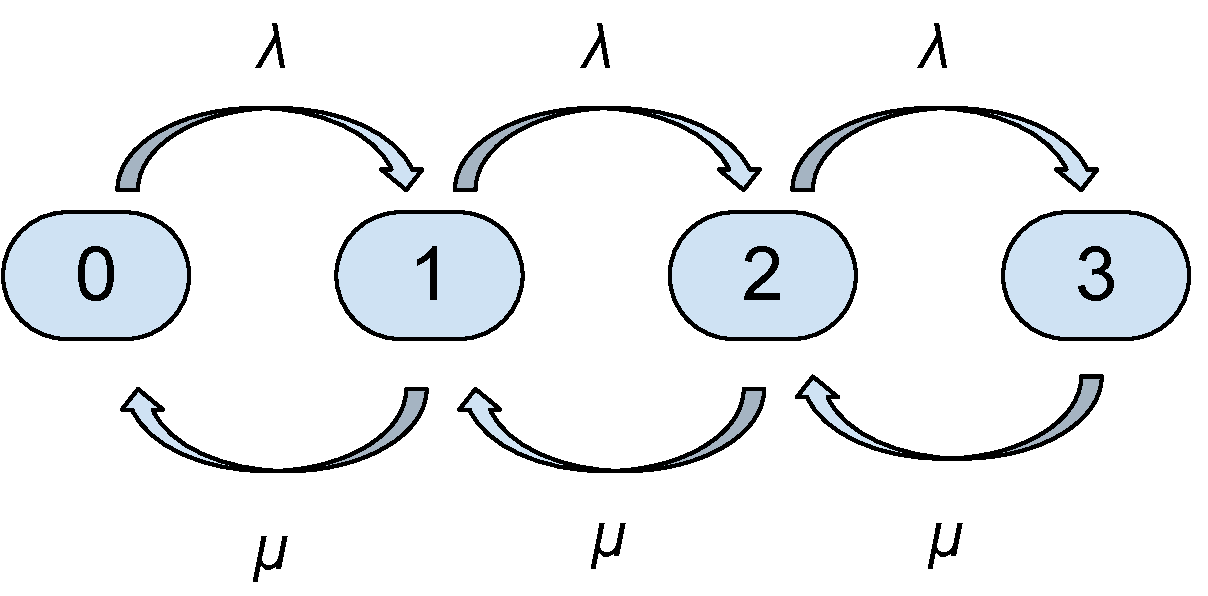
\includegraphics[width=10cm]{exercise_5_markov_chain}
\end{center}
which has rate matrix:
$$\begin{pmatrix}
-\lambda & \lambda & 0&0\\
\mu &-(\lambda + \mu )&\lambda&0\\
0 & \mu &-(\lambda+\mu)&\lambda\\
0 & 0 &\mu&-\mu\\
\end{pmatrix}
$$

The steady state equations are given by:
$$\begin{array}{@{}r@{\;}c@{\;}l@{}}
\pi_0\lambda&=&\pi_1\mu\\[2mm]
\pi_1(\lambda+\mu)&=&\pi_0\lambda+\pi_2\mu\\[2mm]
\pi_2(\lambda+\mu)&=&\pi_1\lambda+\pi_3\mu\\[2mm]
\pi_3\mu&=&\pi_{2}\lambda\\[2mm]
\end{array}$$

The solution for this system can be found (make sure you are able to do this!) to be:

$$\begin{array}{@{}r@{\;}c@{\;}l@{}}
\pi_0&=&{1\over 1+\rho+\rho^2+\rho^3}\\[2mm]
\pi_1&=&\rho\pi_0\\[2mm]
\pi_2&=&\rho^2\pi_0\\[2mm]
\pi_3&=&\rho^3\pi_0\\[2mm]
\end{array}$$

as required. The mean number of vehicles at the station is given by:

$$\begin{array}{@{}r@{\;}c@{\;}l@{}}
\sum_{i=0}^3i\pi_i&=&\sum_{i=0}^3{i\rho^i\over 1+\rho+\rho^2+\rho^3}\\[2mm]
&=&{1\over 1+\rho+\rho^2+\rho^3}\sum_{i=0}^3i\rho^i\\[2mm]
&=&{\rho(1+2\rho+3\rho^2)\over 1+\rho+\rho^2+\rho^3}\\[2mm]
\end{array}$$


\item We have the Markov chain given by

\begin{center}
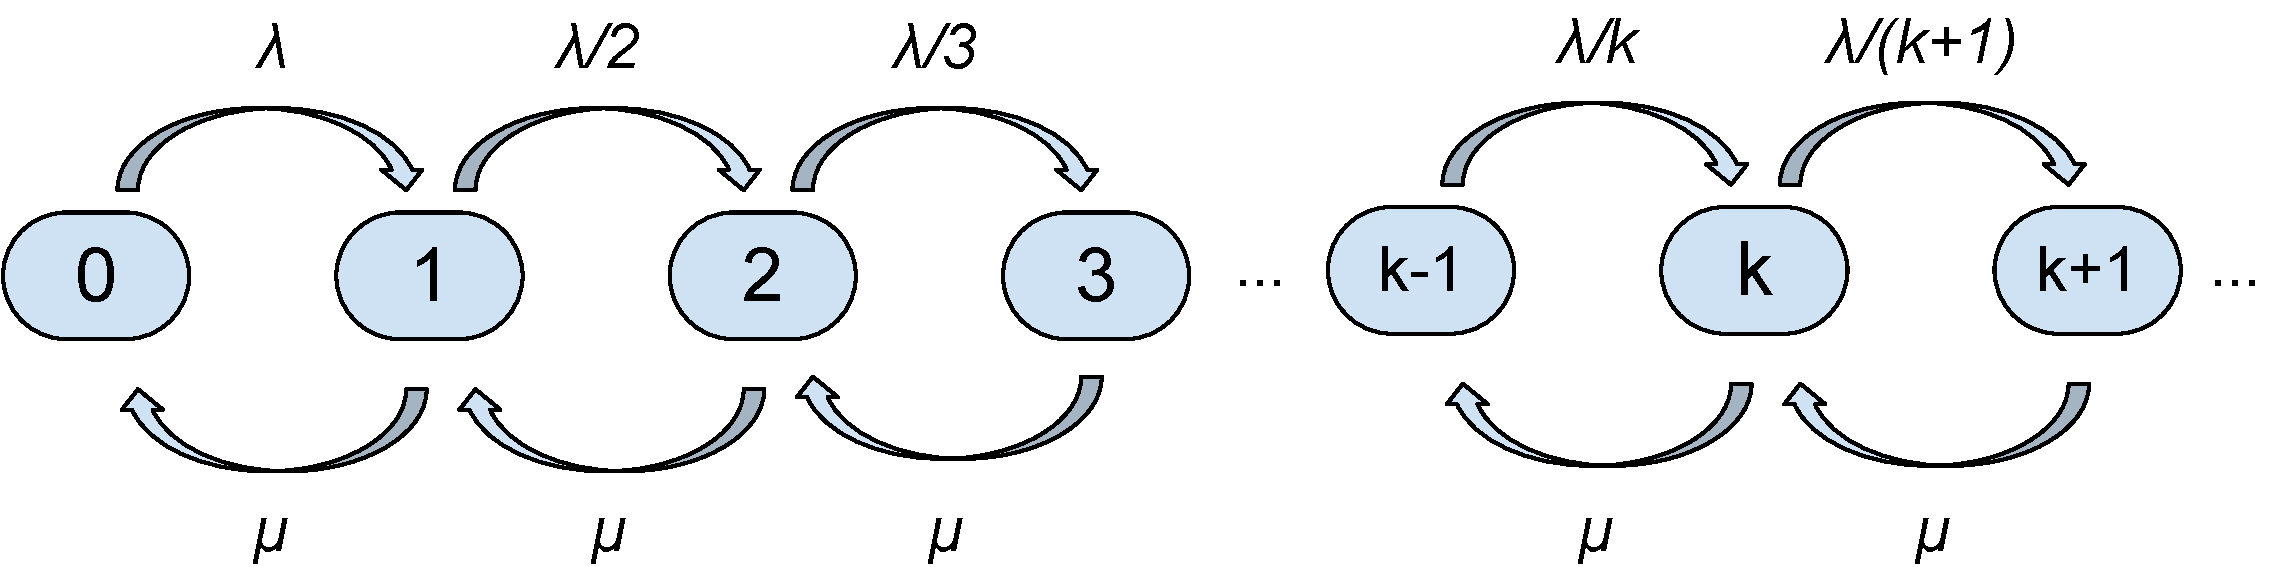
\includegraphics[width=10cm]{exercise_6_markov_chain}
\end{center}

The steady state equations are:
$$\begin{array}{@{}r@{\;}c@{\;}l@{}}
\pi_0\lambda&=&\pi_1\mu\\[2mm]
\pi_1({\lambda\over2}+\mu)&=&\pi_0\lambda+\pi_2\mu\\[2mm]
&\vdots&\\[2mm]
\pi_{i}({\lambda\over k+1}+\mu)&=&\pi_{k-1}{\lambda\over k}+\pi_{k+1}\mu
\end{array}$$

By inspection we have:

$$\begin{array}{@{}r@{\;}c@{\;}l@{}}
\pi_1&=&\rho\pi_0\\[2mm]
\pi_2&=&{\rho^2\over 2}\pi_0\\[2mm]
\pi_3&=&{\rho^3\over 3!}\pi_0\\[2mm]
&\vdots&\\[2mm]
\pi_{k+1}&=&{\rho^{k+1}\over {k+1}!}\pi_0\\[2mm]
\end{array}$$

We conjecture that $\pi_i={\rho^i\over i!}\pi_0\text{ for all }i\geq1$. We prove this by induction. For $i=1$ we have $\pi_1=\rho\pi_0$ as required. Let us know assume that $\pi_i={\rho^i\over i!}\pi_0$ for all $i\leq n$ for some $n\geq 1$. From above we then have:
$$\pi_{n+1}={\pi_{n}({\lambda\over n+1}+\mu)-\pi_{n-1}{\lambda\over n}\over \mu}=\pi_0\left({\rho^n\over n!}\left({\rho\over n+1}+1\right)-{\rho\over n!}\right)={\rho^{n+1}\over (n+1)!}\pi_0$$

as required.

Finally, taking the sum or probabilities equal to 1, we have:
$$\sum_{k=0}^{\infty}{\rho^k\over k!}\pi_0=1\Rightarrow\pi_0=e^{-\rho}$$
thus we have $\pi_i={\rho^i\over i!}e^{-\rho}\text{ for all }i\geq0$.

\item We have $\lambda=5$ and $\mu=6$, thus for the formula for the $M/M/1$ queue we have:
$L_c={\rho\over1-\rho}=5$ which gives an hourly cost of $5+5\times8=\$45\text{ per hour}$.

If a second distribution centre is setup we can expect the arrival rate at each centre to be $\lambda={5\over 2}$. We still have $\mu=6$. The average number of workers at each centre is: $L_c={5\over7}$, thus ${10\over 7}$ overall. This gives an hourly cost of $2\times5+{80\over7}\approx\$21.43\text{ per hour}$. Thus, employing a second distributor is justified.


\item We can use the formulas from question 1 to obtain the following table:


\begin{center}
\begin{tabular}{c|c|c}
         &$M/M/1$&$M/M/2$\\\hline
$\lambda$&.4     &.4     \\
$\mu$    &.8     &.5     \\
$\rho$   &.5     &.4     \\\hline
$\pi_0$  &$(1-\rho)=.5$     &${1-\rho\over1+\rho}={6\over14}\approx.4286$\\
$L_q$&${(.5)^2\over 1-.5}.5$&${2*(.4)^3\over 1-.4^2} \approx.15$\\
$W_q$&${5\over4}= 1.25$&${8\over 21}\approx.38095$\\
$W_c$&  ${5\over2}=2.5$&${50\over 21}\approx2.38095$\\
$L_c$&1&${20\over21}\approx.952381$\\
$P(\text{wait})$&$1-\pi_0={1\over2}$&$1-\pi_0-\pi_1=1-{6\over14}(1+{4\over5})\approx.228570$
\end{tabular}
\end{center}
(The last point uses the fact that $\pi_1={\lambda\over\mu}\pi_0$ in an $M/M/2$ queue.)

From this analysis it could be recommended that the new proposal is implemented. Indeed, this would give a shorter wait to customers ($W_q$ and $P(\text{wait})$).
\end{enumerate}


\end{document} 
